\documentclass[article]{jss}

%%%%%%%%%%%%%%%%%%%%%%%%%%%%%%
%% declarations for jss.cls %%%%%%%%%%%%%%%%%%%%%%%%%%%%%%%%%%%%%%%%%%
%%%%%%%%%%%%%%%%%%%%%%%%%%%%%%

%% almost as usual
\author{Hannes Matuschek\\University of Potsdam, Germany}
\title{\pkg{StochBB}: A Software Framework and Application for Analyzing Networks of Random Variables}

%% for pretty printing and a nice hypersummary also set:
\Plainauthor{Hannes Matuschek} %% comma-separated
\Plaintitle{StochBB: A Software Framework and Application for Analyzing Networks of Random Variables} %% without formatting
\Shorttitle{\pkg{StochBB}: Analyzing Networks of Random Variables} %% a short title (if necessary)

%% an abstract and keywords
\Abstract{
  \pkg{StochBB} is a sofware framework and a graphical user interface program that allows to analyze
complex systems of dependent random variables efficiently. For example, such networks are 
frequently used to describe cognitive processes and are usually analyzed by means of Monte Carlo
type stochastic simulations. Although very flexible, the stochastic simulation approach requires a
large number of samples to be drawn, to obtain reliable statistics for the response variable of
interest. In contrast to stochastic simulation, \pkg{StochBB} derives the marginal distributions of
dependent random variables analytically and resorts to numerical solutions whenever the analytic
approach fails. To achieve this,  \pkg{StochBB} implements a rudimentary computer algebra system
for systems of dependent random variables. As an example, we analyze a simple cognitive model that
with a divergence point.
}
\Keywords{random variables, computer algebra system, stochastic simulation, \proglang{C++}, \proglang{Python}, \proglang{R}}
\Plainkeywords{random variables, computer algebra system, stochastic simulation, C++, Python, R} %% without formatting
%% at least one keyword must be supplied

%% publication information
%% NOTE: Typically, this can be left commented and will be filled out by the technical editor
%% \Volume{50}
%% \Issue{9}
%% \Month{June}
%% \Year{2012}
%% \Submitdate{2012-06-04}
%% \Acceptdate{2012-06-04}

%% The address of (at least) one author should be given
%% in the following format:
\Address{
  Hannes Matuschek\\
  Department of Mathematics\\
  Focus area \emph{Dynamics of Complex Systems}\\
  University of Potsdam\\
  Karl-Liebknecht-Strasse 24-25\\
  D-14476 Potsdam, Germany\\
  E-mail: \email{hannes.matuschek@uni-potsdam.de}\\
}
%% It is also possible to add a telephone and fax number
%% before the e-mail in the following format:
%% Telephone: +43/512/507-7103
%% Fax: +43/512/507-2851

%% for those who use Sweave please include the following line (with % symbols):
%% need no \usepackage{Sweave.sty}

%% end of declarations %%%%%%%%%%%%%%%%%%%%%%%%%%%%%%%%%%%%%%%%%%%%%%%

\usepackage{listings}
\usepackage{amsmath}
%\usepackage{geometry}
\usepackage{color}
%\usepackage{natbib}
\usepackage{graphicx}
\usepackage{subcaption}
\usepackage{editorial}
%\usepackage{codedoc}

\begin{document}

%% include your article here, just as usual
%% Note that you should use the \pkg{}, \proglang{} and \code{} commands.

 \section{Introduction} \label{sec:intro}
Frequently, complex systems are described in terms of stochastic processes, as the
underlying deterministic process is too complex to be modeled exactly or as the
process is indeed random. It is not always the random process itself that is of 
interest, but a derived quantity. For example, the distribution of waiting times until the
process reaches a certain state. In the field of cognitive psychology, random processes are frequently used to
describe each processing stage in a chain of stages that leads to a response. The state of
each random process itself is usually not measurable but the total response time of all processing 
stages involved. Although each processing stage is modeled as a random process, the waiting-time
of a single stage is just a random variable and the complete system is then a system of dependent random 
variables.

StochBB is able to describe and analyze complex systems of dependent random variables
by combining simple ones (representing single stages with a known waiting-time distribution) to
a complex system. For example, consider the following independent random variables
\begin{equation}
  X_1 \sim \Gamma(10, 100)\,, X_2 \sim \Gamma(20, 50)\text{ and } X_3 \sim \text{Exp}(0.01)\,,\nonumber
\end{equation}
which are described completely by their distribution. This means that the time, the
processing stage $X_1$ needs to complete is gamma-distributed with shape $k=10$ and scale
$\theta=100$. Analogously, the stages $X_2$ and $X_3$ are defined by their own waiting-time 
distribution.

From these basic building blocks, a more complex system can be assembled by
combining them. Using the example above, one may define a new processing stage that is a chain of
the stages $X_1,\dots,X_3$. This simple chain then describes the successive
processing of information entering the first stage described by $X_1$.
Once the first processing stage finished, its result gets forwarded to the second stage described
by $X_2$ and finally to the last stage described by $X_3$. The waiting time of the
complete chain is again a random variable that is the sum of all random variables,
or expressed mathematically
\begin{equation}
 Y = X_1 + X_2 + X_3\,. \nonumber
\end{equation}

SochBB determines the probability density function (PDF) or cumulative probability function
(CDF) of the waiting-time distribution of the process $Y$ analytically (as far as
possible) or resorts to a numeric method if the analytic approach fails. More over it provides an efficient
and correct sampler for the system of random variables.


\section{Representation and reductions of random variables}
Continuing the example above, please note that the sum of random variables commutes. Hence the
random variable $Y$ remains the same if defined as $Y = X_1 + X_3 + X_2$ instead of 
$Y = X_1 + X_2 + X_3$. Moreover, the 
distribution of the sum of $X_1$ and $X_3$ can be determined analytically as 
$X' = (X_1+X_3)\sim\Gamma(11,100)$. Hence the random variable $Y$ can now be expressed as 
$Y = X_2 + X'$, and only a single numeric convolution is necessary to obtain the PDF of the
random variable $Y$. 

StochBB implements several reductions of the system of random variables,
exploiting mathematical identities of random variables. To this end, it allows to obtain the PDFs and CDFs
of random variables efficiently.

\subsection{Affine transformations of random variables}
An affine transformation of the random variable $X$ has the form $Y = a\,X+b$, where $a\neq 0$
and $b$ are real values. Although affine transformations of random variables are not frequently
used directly in a system of random variables, they may appear as a result of other reductions
of the system. The PDF and CDF of the random variable $Y$ defined above, are then 
\begin{equation}
 f_Y(y) = \frac{1}{a}f_X\left(\frac{y-b}{a}\right)\text{ and }
 F_Y(y) = F_X\left(\frac{y-b}{a}\right)\,. \nonumber
\end{equation}

Of course, an affine transformation of an affine transformed random variable $X$ is also a simple 
affine transformation of the random variable. Hence the following reduction is implemented
\begin{equation}
 c\,(a\,X+b)+d \longrightarrow (a\,c)\,X+(c\,b+d)\,.\nonumber
\end{equation}

\subsection{Sums of random variables}
Sums of random variables have been introduced briefly above and may represent a chain of processing
stages being triggered sequentially. The sum itself is a derived random variable that depends on all
mutually independent variables being summed up. The PDF of the sum $Y$ is then the convolution of all
PDFs of the summed variables. That is
\begin{align}
 Y &= \sum_{i=0}^NX_i\text{ where } X_i \sim f_i(x)\text{ mutually independent} \nonumber \\
 Y &\sim f_1(x) \ast \cdots \ast f_N(x)\,. \nonumber
\end{align}

The direct numerical convolution of the underlying distributions can be computationally expensive if the
number of PDFs is large. Assuming that all distributions are well supported on a common interval, however, 
allows for a fast numerical convolution by means of FFT convolution \cite{Press2007}. For the FFT convolution, all 
densities $f_i(x)$ are evaluated on a common regular gird and the evaluation of the convolution on that gird
can then be computed easily. This, however, requires that the grid is chosen such that all densities being
convoluted as well as the result are well supported on the chosen interval. Moreover, the grid must be fine 
enough to capture the details of all distributions. 

The numerical convolution, like any numerical approach, is only an approximation. Hence StochBB tries to perform
the convolutions analytically before resorting to the numerical approach. 

First all sums of random variables are flattened. That is, 
\begin{equation}
 \begin{array}{l}
  Y_1 = X_1 + X_2\\
  Y_2 = Y_1 + X_3 
 \end{array} \longrightarrow 
 \begin{array}{l}
  Y_1 = X_1 + X_2\\
  Y_2 = X_1 + X_2 + X_3 
 \end{array}\,. \nonumber
\end{equation}

Then, the distribution of the sum is derived. Here the following reductions are performed.
\begin{align}
 \delta(x-x_0)\ast U[a,b](x) &\longrightarrow U[a+x_0,b+x_0](x)\,, \nonumber \\
 \delta(x-x_0)\ast \phi(x; \mu, \sigma) &\longrightarrow \phi(x; \mu+x_0, \sigma)\,, \nonumber \\
 \phi(x; \mu_1, \sigma_1)\ast \phi(x; \mu_2, \sigma_2) &\longrightarrow 
   \phi(x; \mu_1+\mu_2, \sqrt{\sigma_1^2+\sigma_2^2}) \nonumber\,, \\
 \Gamma(x; k_1, \theta)\ast \Gamma(x; k_2, \theta) &\longrightarrow 
   \Gamma(x; k_1+k_2, \theta)\,, \nonumber
\end{align}
where $\delta(\cdot-x_0)$ is the delta distribution located at $x_0$, $U[a,b](\cdot)$ the uniform
distribution on the interval $[a,b]$, $\phi(\cdot; \mu, \sigma)$ the normal distribution with mean 
$\mu$ and standard deviation $\sigma$ and $\Gamma(\cdot; k, \theta)$ the gamma distribution with
shape $k$ and scale $\theta$.

\subsection{Minimum and maximum of random variables}
The minimum or maximum of some given random variables, e.g. $Y=\min\{X_1,X_2\}$ or 
$Y=\max\{X_1,X_2\}$ are them self random variables. These derived random variables can be used to
express the waiting time of a processing stage that consists of several independent processes being
performed in parallel (in contrast to sequential processes described by sums of random variables). 
If the processing stage finishes once the first of the parallel processes finishes, the 
resulting waiting time can be expressed by the minimum of the underlying random variables. If the stage
finishes once all underlying processes are finished, the resulting waiting time can be described
by the maximum.	 

If the two independent random variables $X_1$ and $X_2$ are distributed according to the (cumulative) distribution
functions $F_1(x)$ and $F_2(x)$, the maximum of these two random variables $Y=\max\{X_1,X_2\}$
is distributed according to the probability function $F_Y(y)=F_1(y)\cdot F_2(y)$. Consequently, its PDF
is $f_Y(y)=f_1(y)\cdot F_2(y) + f_2(y)\cdot F_1(y)$, where $f_1(\cdot)$ and $f_2(\cdot)$ are the PDFs
of the random variables $X_1$ and $X_2$. Likewise, the CDF and PDF of the minimum can be expressed as
$F_Y(y)=1-(1-F_1(y))\cdot(1-F_2(y))$ and therefore $f_Y(y) = f_1(y)(1-F_2(y)) + f_2(y)(1-F_1(y))$.

For applying these equations to derive the CDF and PDFs of the minimum and maximum random variables, the 
underlying random variables must be independent. To achieve independence where possible, the following 
reductions are performed on maximum as well as minimum random variables.

Again, first maximum and minimum structures were flattened, for example
\begin{equation}
 \begin{array}{l}
  Y_1 = \max\{X_1,X_2\}\\
  Y_2 = \max\{Y_1,X_3\}
 \end{array} \longrightarrow
 \begin{array}{l}
  Y_1 = \max\{X_1,X_2\}\\
  Y_2 = \max\{X_1,X_2,X_3\}
 \end{array}\,, \nonumber
\end{equation}
then, possible common terms are collected like
\begin{equation}
 \max\{X_1 + X_2, X_3 + X_2\} \longrightarrow \max\{X_1,X_3\}+X_2\,. \nonumber
\end{equation}

The latter transformation does not ensure independence of random variables, but 
decreases the complexity of setting-up a complex system of random variables by 
resolving simple-structured dependencies between random variables.

\subsection{Mixture of random variables}
A mixture is the weighted sum of random variables
\begin{equation}
 Y = \frac{w_1X_1+\cdots+w_NX_N}{w_1+\cdots+w_N}\,, \nonumber
\end{equation}
where $w_i$ are positive weights. The result $Y$ is also a random variable with the PDF
\begin{equation}
 f_Y(y) = \frac{w_1f_1(x)+\cdots+w_Nf_N(x)}{w_1+\cdots+w_N}\,,\nonumber
\end{equation}
where $f_i(\cdot)$ is the PDF of the i-th random variable $X_i$. The CDF of the
mixture is obtained analogously. A mixture can be used to describe a random 
path-selection in a system of processing stages. 

\subsection{Conditional random variables}
The \emph{conditional} random variable selects one of two random variables (e.g. $Y_1$ or $Y_2$) depending
on the condition $X_1 < X_2$. That is 
\begin{equation}
 Z = \begin{cases}
   Y_1 & \mbox{if } X_1 < X_2\\
   Y_2 & \mbox{else\,,} 
 \end{cases} \nonumber
\end{equation}
where $X_1, X_2, Y_1$ and $X_1, X_2, Y_2$ are mutually independent random variables. The variables
$Y_1$ and $Y_2$ do not need to be mutually independent. Given that the possible result variables $Y_1$
and $Y_2$ are independent from the condition, the result variable is then a simple mixture where the weight
is given by the probability of $X_1<X_2$. Hence the density of the result variable $Z$ is
\begin{align}
 f_Z(z) &= Pr[X_1<X_2]\,f_{Y_1}(z) + \left(1-Pr[X_1<X_2]\right)\,f_{Y_2}(z) \nonumber \\
    &= f_{Y_1}(z)\,\int_{-\infty}^{\infty}F_{X_1}(x)\,f_{X_2}(x)\,dx + 
    f_{Y_2}(z)\,\int_{-\infty}^{\infty}F_{X_2}(x)\,f_{X_1}(x)\,dx\,.\nonumber
\end{align}

\subsection{Conditional chained random variables}
One of the few non-textbook examples of a derived random variable is the conditional chained random variable. 
It can be defined as
\begin{equation}
 Z = \begin{cases}
   X_1 + Y_1 & \mbox{if } X_1 < X_2\\
   X_2 + Y_2 & \mbox{else\,,} 
 \end{cases} \nonumber
\end{equation}
where $X_1, X_2, Y_1$ and $X_1, X_2, Y_2$ are mutually independent. $Y_1$ and $Y_2$ may be 
dependent random variables. Although being similar to the conditional random variable, there is an 
important difference: Both possible outcomes ($X_1+Y_1$ and $X_2+Y_2$) 
are not independent from the condition (i.e. $X_1+Y_1$ depends trivially on $X_1$).
Therefore, the simple conditional random variable cannot be used here. 

The conditional chained random variable can be used to describe two independent parallel processing
stages where the fastest stage will trigger another stage. For example, if $X_1$ wins, it triggers $Y_1$
and if $X_2$ wins it triggers $Y_2$. In contrast to the conditional chained random variable, the 
conditional random variable does not trigger a third stage but \emph{selects} the value of a third stage. 
Therefore, the actual waiting time of the \emph{winning} stage does not have an influence on the 
selected one and may lead to non-causal waiting times if $X_1$ and $X_2$ are larger than $Y_1$ and
$Y_2$ (i.e., the response is faster than the processes selecting the response). The conditional chained 
random variable always maintains causality.  	

The conditional	 chained random variable is certainly not common and to my knowledge not
covered in text books. Hence the density for it must be obtained first.
Given that the cases ($X_1<X_2$ and $X_2<X_1$) are mutually exclusive, the density of $Z$, 
$f_Z(z)$ can be expressed as a simple sum. Precisely
\begin{multline}
 f_Z(z) = \iiint_{-\infty}^\infty f(x_1,x_2,y_1|z=x_1+y_1,x_1<x_2)\,dx_1\,dx_2\,dy_1 \\
  + \iiint_{-\infty}^\infty f(x_1,x_2,y_2|z=x_2+y_2,x_2<x_1)\,dx_1\,dx_2\,dy_2\,. \nonumber
\end{multline}

Given that $X_1, X_2$ and $Y_1$ are mutually independent, the first integral can be reduced to
\begin{multline}
\iiint_{-\infty}^\infty f(x_1,x_2,y_1|z=x_1+y_1,x_1<x_2)\,dx_1\,dx_2\,dy_1 \\
  = \iiint_{-\infty}^\infty f_{X_1}(x_1)\,f_{X_2}(x_2)\,f_{Y_1}(y_1)\,\delta(z-x_1-y_1)\,H(x_2-x_1)\,dx_1\,dx_2\,dy_1\\
  = \iint_{-\infty}^\infty f_{X_1}(x_1)\,f_{X_2}(x_2)\,f_{Y_1}(z-x_1)\,H(x_2-x_1)\,dx_1\,dx_2\\
  = \int_{-\infty}^\infty f_{X_1}(x_1)\,f_{Y_1}(z-x_1)\int_{-\infty}^\infty \,f_{X_2}(x_2)\,H(x_2-x_1)\,dx_2\,dx_1\\
  = \int_{-\infty}^\infty f_{X_1}(x_1)\,f_{Y_1}(z-x_1)\int_{x_1}^{\infty} \,f_{X_2}(x_2)\,dx_2\,dx_1\\
  = \int_{-\infty}^\infty f_{X_1}(x_1)\,\left(1-F_{X_2}(x_1)\right)\,f_{Y_1}(z-x_1)\,dx_1\,. \nonumber
\end{multline}

Analogously, the second integral can be reduced to
\begin{multline}
\iiint_{-\infty}^\infty f(z,x_1,x_2,y_2|z=x_2+y_2,x_2<x_1)\,dx_1\,dx_2\,dy_2 \\
 = \int_{-\infty}^\infty \,f_{X_2}(x_2)\left(1-F_{X_1}(x_2)\right)\,f_{Y_2}(z-x_2)\,dx_2\,. \nonumber
\end{multline}

The final density of $Z$ is then given by
\begin{multline}
 f_Z(z) = \int_{-\infty}^\infty f_{X_1}(x_1)\,\left(1-F_{X_2}(x_1)\right)\,f_{Y_1}(z-x_1)\,dx_1\nonumber \\
  + \int_{-\infty}^\infty \,f_{X_2}(x_2)\left(1-F_{X_1}(x_2)\right)\,f_{Y_2}(z-x_2)\,dx_2\,, \nonumber \\
  = \left[f_{X_1}\,\left(1-F_{X_2}\right)\right]\ast f_{Y_1} 
       + \left[f_{X_2}\left(1-F_{X_1}\right)\right]\ast f_{Y_2}\,,\nonumber
\end{multline}
and it can be evaluated using the same \emph{trick} used for chains of random variables.

\subsection{Compound random variables}
The most complex derived random-variable type is the compound random variable. That is a random variable
$X$ distributed according to a parametric distribution $X\sim f_{X|A}(x;A)$ with parameter $A$. $A$, however, 
is itself a random variable with its own distribution $A\sim g(a)$. The distribution of the compound 
random variable $X$ is then obtained by marginalizing the parameter of the PDF $f_{X|A}(\cdot;a)$ as 
\begin{equation}
 f_X(x) = \int f_{X|A}(x;a)\,g(a)\,da\,,\nonumber
\end{equation}
and the CDF is obtained analogously as
\begin{equation}
 F_X(x) = \int F_{X|A}(x;a)\,g(a)\,da\,.\nonumber
\end{equation}

StochBB determines the PDF and CDF of $X$ by performing the integral numerically.


\section{Software Architecture}
In this section, I briefly describe the software architecture of the complete \pkg{StochBB} framework as shown in Fig. \ref{fig:arch}. 

\begin{figure} [!ht]
 \centering
 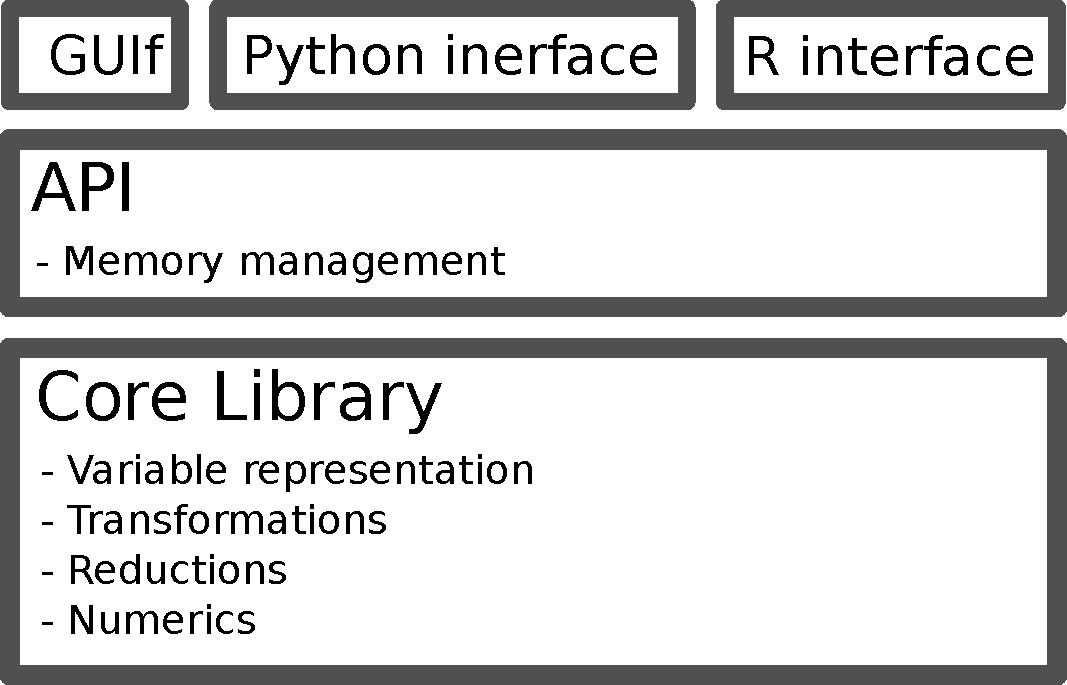
\includegraphics[width=0.5\textwidth]{fig/arch.pdf}
 \caption{Overview of the \pkg{StochBB} software architecture.} \label{fig:arch}
\end{figure}

The foundation of the complete framework is formed by the \pkg{StochBB} core library. This C++ library implements the core functionality of the system. Prominent elements are classes representing the atomic random-variable instances and parametric distributions as well as derived variables (e.g., sums of random variables) and their distributions (e.g., convolution densities).  Together, these classes form the representation of a complex system of dependent random variables. Analytic solutions for some marginal distributions are obtained by reduction and transformation operations performed on the system representation. Also these operations are part of the core library. Finally a set of numerical algorithms (e.g., numerical convolution and integrals) are implemented in the core library for obtaining numerical approximations of densities which cannot be derived analytically. 

Using the core library directly would be rather complicated as the C++ does not provide means of automatic memory management by itself. For easing the usage of the core library an application programming interface is provided above the core library that encapsulates all objects of the core library into container classes. These container classes then implement an automatic memory management by means of a \emph{mark-and-sweep} garbage collector \cite[e.g.,][]{Aho2007}. This API (described in the next section) is then used to provide interfaces to the Python and R programming language as well as implementing a graphical user interface (GUI) application also described below.
\section{Application programming interface} \label{sec:api}
The application programming interface (API, see also \cite{stochbbapi}) 
allows to assemble complex systems of random variables programmatically in C++.
All API classes are derived from the \class{Container} class which is an essential part of the
memory management system used by StochBB. Usually the C++ programmer needs to keep track of all
objects still in use and is responsible to free unneeded objects to avoid memory leaks. This can
be a difficult task when dealing with complex structured objects cross-referencing each other.
To ease the usage of StochBB, a \emph{mark and sweep} garbage collector is implemented which keeps track
of all objects being directly or indirectly reachable and freeing all unreachable objects. For
this memory management system to work, it is necessary to treat all container objects like values
although they represent references to objects allocated on the heap.

There is also a Python package (called \code{stochbb}) that exposes the classes and functions 
of the C++ API to python. This allows for a convenient construction of systems of random variables
while maintaining the speed of the C++ classes. The Python API is almost identical to the C++ one
described below except that \code{numpy} array are used in Python instead of Eigen matrices and 
vectors.

The central class of StochBB is \class{Var}, representing a random variable. This could be a
simple random variable having a specified distribution (see \class{AtomicVar}) or a random
variable that is derived from others like \class{Chain}, \class{Minimum}, \class{Maximum} or
\class{Mixture}. All random variables (atomic and derived) have probability density functions
attached. They can be accessed using the \method{Var}{density} method which returns a 
\class{Density} object.

All \class{Density} objects have two methods, \method{Density}{eval} evaluating the probability
density function and \method{Density}{evalCDF} evaluating the cumulative density or probability
function. Assembling a system of random variables and evaluate their PDFs or CDFs is straight
forward. Sampling, however, is not that trivial and is described below in some detail.

\subsection{Assembling a system of random variables}
In a first step, one may define a new gamma-distributed random variable with shape $k=10$
and scale $\theta=100$ as
\begin{lstlisting}[language=C++]
 #include <stochbb/api.h>
 using namespace stochbb;
 
 // [...]
 
 Var X1 = stochbb::gamma(10, 100);
\end{lstlisting}

Its PDF can then be evaluated as on a regular grid in $[0,1000)$ with $1000$ grid points as
\begin{lstlisting}[language=C++]
 // [...]
 
 Eigen::VectorXd pdf(1000);
 X1.density().eval(0, 1000, pdf);
\end{lstlisting}

The result of the evaluation is stored into the vector \code{pdf}. There are only very few basic
or atomic random-variable types defined in StochBB:

\begin{tabular}{l|l|l}
 Constructor & Parameters & Process description \\ \hline
 \function{stochbb::delta} & \code{delay} & A constant delay or a process with a fixed waiting time. \\
 \function{stochbb::unif} & \code{a}, \code{b} & A process with a uniform-distributed waiting time. \\
 \function{stochbb::norm} & \code{mu}, \code{sigma} & A process with a normal-distributed waiting time. \\
 \function{stochbb::gamma} & \code{k}, \code{theta} & A process with a gamma-distributed waiting time. \\
 \function{stochbb::weibull} & \code{k}, \code{lambda} & A process with a Weibull-distributed waiting time. \\
\end{tabular}

More complex processes can be derived by combining these atomic random variables or as special cases of them.


\subsubsection{Affine transformation of random variables}
An affine transformation of the random variable $X$ is of the form $a\,X+b$, where $a\neq 0$ and $b$ are
real values. An affine transformation can be obtained using the overloaded * and + operators or using the
\function{stochbb::affine} function. For example, the code
\begin{lstlisting}[language=C++]
 #include <stochbb/api.h>
 using namespace stochbb;
 
 // [...]
 
 Var X = stochbb::gamma(10, 100);
 Var Y = 3*X + 1;
\end{lstlisting}
constructs a random variable \code{Y} being an affine transformed of the random variable \code{X}.

\subsubsection{Sums of random variables}
Beside the affine transfrom of random variables, the most basic derived random variable is a \class{Chain}.
This type represents the \emph{chaining} of random processes. Such a chain can be constructed using 
the overloaded \code{+} operator or the \function{stochbb::chain} function. For example
\begin{lstlisting}[language=C++]
 #include <stochbb/api.hh>
 using namespace stochbb;

 // [...]

 Var X1 = stochbb::gamma(10,100);
 Var X2 = stochbb::gamma(20, 50);
 Var Y = X1 + X2;
\end{lstlisting}

\subsubsection{Minimum and Maximum of random variables}
Another simple derived random variable is the \class{Maximum} or \class{Minimum} class. As the
names suggest, they represent the maximum or minimum of a set of random variables. They can be
created using the overloaded standard library function \code{std::min} and \code{std::max} or the
\function{stochbb::minimum} and \function{stochbb::maximum} functions. The latter take a vector of random variables.
\begin{lstlisting}[language=C++]
 #include <stochbb/api.hh>
 using namespace stochbb;

 // [...]

 Var X1 = stochbb::gamma(10,100);
 Var X2 = stochbb::gamma(20, 50);
 Var Y = std::max(X1, X2);
\end{lstlisting}

\subsubsection{Mixtures of random variables}
Similar to the \class{Minimum} or \class{Maximum}, a mixture of random variables can be
constructed using the \function{stochbb::mixture} function. This function takes a at least 
two variables and their associated weight. Such a mixture can be considered as a random process which
randomly selects the outcome of a set of other random processes, where the probability of
selecting a specific process is given by the relative weight assigned to each process.
\begin{lstlisting}[language=C++]
 #include <stochbb/api.hh>
 using namespace stochbb;

 // [...]

 Var X1 = stochbb::gamma(10,100);
 Var X2 = stochbb::gamma(20, 50);
 Var Y = stochbb::mixture(1,X1, 2,X2);
\end{lstlisting}

In the example above, the random process $Y$ will select the outcome of $X_1$ with
a probability of $\frac{1}{3}$ and the outcome of $X_2$ with probability
$\frac{2}{3}$.

\subsubsection{Compound random variables}
An important class of derived random processes are compound processes. There the parameters of the
distribution of a random variable are themselves random variables. That is
\begin{equation}
 X \sim f(x|A)\,,\quad A \sim g(a|\theta)\,, \nonumber
\end{equation}
where the random variable $X$ is distributed as $f(x|A)$, parametrized by $A$,
where $A$ itself is a random variable distributed as $g(a|\theta)$, parametrized by
$\theta$. 

Compound random variables are created using the same factory function like the atomic random variable
types. In contrast to the atomic random variables, the factory functions take random variables as 
parameters instead of constant values.
\begin{lstlisting}[language=C++]
 #include <stochbb/api.hh>
 using namespace stochbb;
 
 // [...]
 
 Var mu = stochbb::gamma(10,100);
 Var cnorm = stochbb::norm(mu, 10);
\end{lstlisting}
instantiates a compound-normal distributed random variable, where the mean is gamma distributed
while the standard deviation is fixed.

\subsection{Sampling several dependent random variables}
As mentioned above, sampling efficiently from a complex system of random variables is not trivial. 
First of all, it must be ensured that all atomic random variables are samples only once. Otherwise, two dependent
random variables may be sampled as independent. Moreover, the results of derived random variables
should be cached for efficiency. 

StochBB provides a separate class that implements a proper sampler for a system
of random variables, the \class{ExactSampler} class. This class allows to sample
from several possibly dependent random variables simultaneously. Upon construction,
the set of random variables to sample from, is specified. A sample from these random
variables can then be obtained by the \method{ExactSampler}{sample} method.
\begin{lstlisting}[language=C++]
 #include <stochbb/api.hh>
 using namespace stochbb;

 // [...]

 Var X1 = stochbb::gamma(10,100);
 Var X2 = stochbb::gamma(20, 50);
 Var Y = std::min(X1, X2);
 // Construct sampler
 ExactSampler sampler(X1, X2, Y);
 // Get 1000 samples
 Eigen::MatrixXd samples(3, 1000);
 sampler.sample(samples);
\end{lstlisting}

The \method{ExactSampler}{sample} method takes a reference to a \class{Eigen::Matrix} where each column
represents the random variable given to the constructor and each row an independent sample from
the system.

For very large systems, sampling may get slow. Particularly if one is only interested
in the marginal distribution of single random variables. For these cases, an approximate sampler
for single random variables is provided, the \class{MarginalSampler}. This sampler uses an
approximation of the inverse of the cumulative distribution function of a random variable
to draw samples.
\begin{lstlisting}[language=C++]
 #include <stochbb/api.hh>
 using namespace stochbb;

 // [...]

 Var X1 = stochbb::gamma(10,100);
 Var X2 = stochbb::gamma(20, 50);
 Var Y = std::min(X1, X2);
 // Sample from Y on [0,500] in 1000 steps
 MarginalSampler sampler(Y, 0, 500, 1000);
 // Get 1000 samples
 Eigen::VectorXd samples(1000);
 sampler.sample(samples);
\end{lstlisting}

In this example, a \class{MarginalSampler} is constructed for the random variable \code{Y}. Using an
approximation of its CDF on the interval $[0,500)$ using $1000$ steps. Then, the
\method{MarginalSampler}{sample} method is used to obtain $1000$ independent samples.



\section{Divergence point example}
This example shows a simple \emph{toy model} for some cognitive process that is able to produce a
so called \emph{divergence point} \cite{Reingold2012}. A divergence point of two response-latency
distributions is the earliest time point at which the two response-latency distributions differ. Obviously, 
there exists no divergence point, if the two response latency distributions are analytic 
(e.g., the convolution of Gamma distributions, \cite{Gelooven1999}). This example, however,
not only shows how a non-analytic response-latency distribution may arise that allows for a 
divergence point, but actually has a divergence point%
\footnote{At least one distribution being non-analytic is a necessary but not a sufficient
condition for the existence of a divergence point.}. 

This very simple model consists of 3 Gamma-distributed random variables $C, X_1$ and $X_2$,
where the latter is a shifted Gamma distribution (here shifted by $300$ ms, i.e. 
$X_3 \sim \Gamma(T-300; k, \theta)$).  The model is
\begin{align}
 \text{control: } & R_c = C + X_1 & \text{ where } C \sim \Gamma(c; 3, 20),\,X_1\sim\Gamma(x_1; 10,30)\\
 \text{experimental: } & R_e = C + \min(X_1, X_2) & \text{ where } X_2 \sim\Gamma(x_2-300; 1, 70)\,.
\end{align}

This model can be read as: Under control condition, the stimulus triggers a common stage $C$ which then 
triggers a second stage $X_2$ that itself immediately triggers the response. Under experimental condition,
again the stimulus triggers the common stage $C$ which then triggers $X_1$. Additionally, the common
stage $C$ also triggers the delayed stage $X_2$ in parallel to $X_1$. The response is then triggered by 
either $X_1$ or $X_2$, depending on which stage completes first. Consequently, the response latency
under control condition is $R_e = C + \min(X_1,X_2)$.

The following code shows how this simple model is implemented using the Python API of StochBB.

\begin{lstlisting}[language=Python]
from numpy import *
import stochbb;

# Processing model
d = 300
C = stochbb.gamma(3,20)
X1 = stochbb.gamma(10,30)
# shifted exponential
X2 = stochbb.gamma(1,70) + d

# response latency control condition
#   is simply R = C + X1
Rc = C + X1
# and for the experimental condition
Re = C + stochbb.minimum(X1, X2)

# Eval PDF & CDF
Tmin, Tmax, N = 0, 1200, 1200;
Tc = empty((N,)); Rc.density().eval(Tmin, Tmax, Tc)
Te = empty((N,)); Re.density().eval(Tmin, Tmax, Te)
TCc = empty((N,)); Rc.density().evalCDF(Tmin, Tmax, TCc)
TCe = empty((N,)); Re.density().evalCDF(Tmin, Tmax, TCe)
\end{lstlisting}

\begin{figure} [!ht]
 \centering
 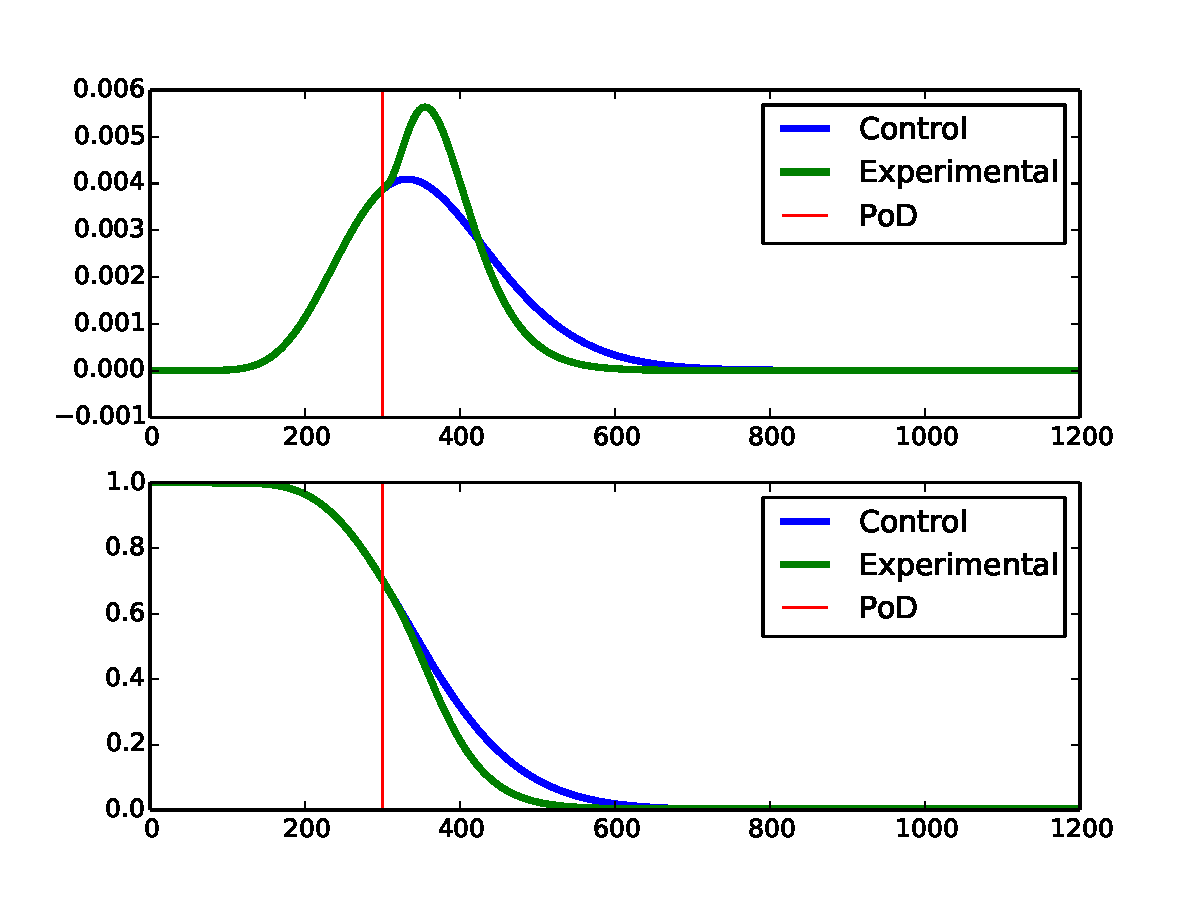
\includegraphics[width=.6\textwidth]{pod.pdf}
 \caption{PDFs (upper panel) and survival functions (lower panel) of the response latencies under 
 control condition (blue lines) and experimental condition (green lines).  The divergence point of 
 the two response-latency distributions is shown as the red vertical lines. \label{fig:pod}}
\end{figure}

Figure \ref{fig:pod} shows the plots generated from the code above. The blue lines show the PDF
(upper panel) and survival function (1-CDF, lower panel) of the response latency under control
condition. Being a convolution of two Gamma distributions, it is an analytic function on the
interval $(0,\infty)$ \citep{Gelooven1999}. The green lines show the PDF and survival function
of the response latency under control condition. As the distribution of $X_2$ is not analytic on the complete interval
$(0,\infty)$ (discontinuity at $T=300$ ms), a divergence point may exist at $T=300$ (red vertical
lines).  In fact, that point is visible in both the PDF and the survival function. Hence, this simple
model is able to produce a divergence point as both response-latency distributions are identical
on the interval $[0,300)$ and diverge thereafter.
	

\bibliography{references}

\end{document}
